\clearpage
\section{Mô hình hóa nâng cao} 
\subsection{Lựa chọn kỹ thuật}
%Giới thiệu thuật toán học máy tập hợp (Ensemble Learning) - Random Forest Regressor đa biến.
Trong giai đoạn mô hình hóa nâng cao, chúng em lựa chọn Random Forest Regressor – một thuật toán thuộc nhóm Ensemble Learning. Random Forest hoạt động bằng cách xây dựng nhiều cây quyết định (Decision Trees) trên các tập dữ liệu con khác nhau, sau đó kết hợp kết quả dự đoán của chúng để đưa ra giá trị cuối cùng
\subsubsection{Cơ sở lựa chọn:}
\begin{itemize}
    \item[-] \textbf{Khả năng nắm bắt quan hệ phi tuyến tính:} Khác với hồi quy tuyến tính đơn giản, Random Forest có thể mô hình hóa các mối quan hệ phức tạp và phi tuyến tính giữa nhiều đặc trưng và giá nhà.
    \item[-] \textbf{Giảm thiểu overfitting:} Nhờ cơ chế bootstrap sampling và bagging, Random Forest thường ổn định hơn so với một cây quyết định đơn lẻ.
    \item[-] \textbf{Khai thác đa biến:} Mô hình cho phép sử dụng nhiều đặc trưng cùng lúc (ví dụ: OverallQual, TotalSF, GrLivArea, các biến log-transform), từ đó tận dụng tối đa thông tin trong dữ liệu.
    \item[-] \textbf{Phân tích độ quan trọng đặc trưng (Feature Importance):} Random Forest cung cấp thước đo định lượng cho thấy đặc trưng nào ảnh hưởng mạnh nhất đến giá nhà, giúp mô hình vừa chính xác vừa dễ diễn giải.
\end{itemize}
\subsubsection{Ý nghĩa học thuật:}
\begin{itemize}
    \item[-] Việc lựa chọn Random Forest thể hiện bước chuyển từ mô hình cơ sở đơn giản sang mô hình nâng cao, có khả năng cải thiện đáng kể độ chính xác.
    \item[-] Đây là một trong những thuật toán phổ biến và mạnh mẽ nhất trong các bài toán dự đoán giá nhà.
\end{itemize}

\subsection{Quá trình huấn luyện}
%Các thiết lập tham số và quá trình fit mô hình.
\subsubsection{Thiết lập tham số:}
\begin{itemize}
    \item[-] Mô hình được khởi tạo với RandomForestRegressor gồm 100 cây quyết định (decision tree) (\verb|n_estimators = 100|).
    \item[-] Sử dụng \verb|random_state = 42| để đảm bảo tính tái lập kết quả.
    \item[-] Tham số \verb|n_jobs = -1| cho phép tận dụng toàn bộ lõi CPU để tăng tốc độ huấn luyện.
\end{itemize}
\subsubsection{Quá trình huấn luyện:}
\begin{figure}[H]
    \centering
    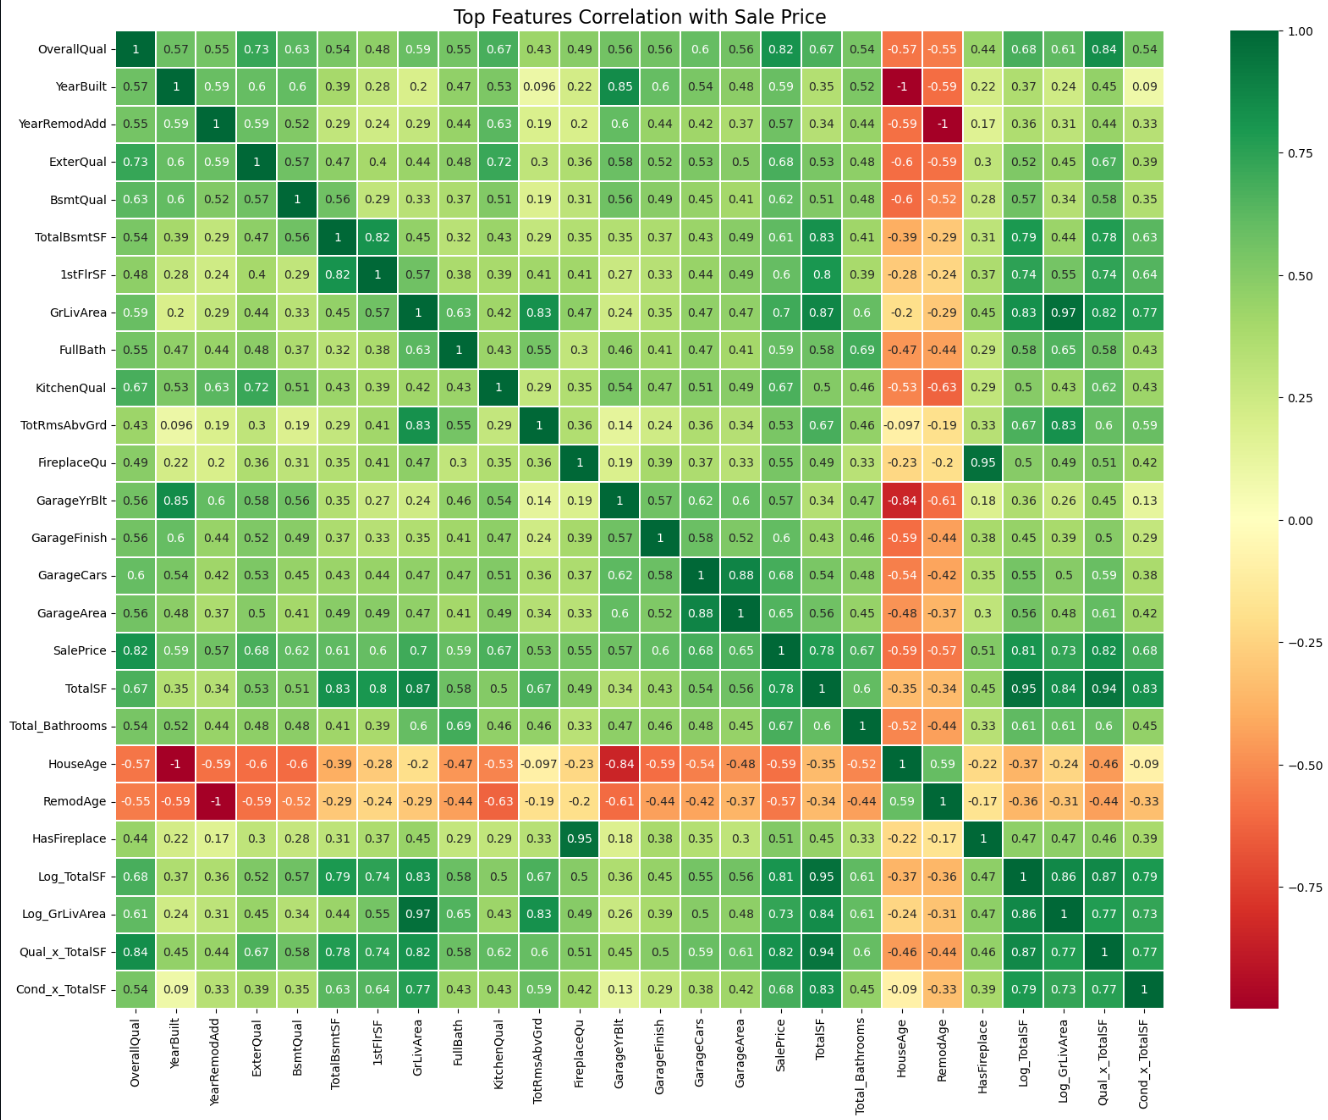
\includegraphics[width=1\linewidth]{images/baseline_model/Heatmap.png}
    \caption{Heatmap tương quan giữa các thành phần với SalePrice}
\end{figure}
\begin{enumerate}
    \item \textbf{Chọn đặc trưng:} Dựa trên phân tích tương quan, chúng tôi lựa chọn các biến có hệ số tương quan cao với SalePrice như:
    \begin{itemize}
        \item[-] Qual\_x\_TotalSF (0.82)
        \item[-] Log\_GrLivArea (0.73)
        \item[-] Log\_TotalSF (0.81)
        \item[-] TotalSF (0.78)
        \item[-] GrLivArea (0.7)
        \item[-] OverallQual (0.82)
    \end{itemize}
    \item \textbf{Chia tập dữ liệu:} Sau đó tiến hành tách dữ liệu ra thành Training và Validation set để đưa vào mô hình huấn luyện.
\end{enumerate}
\begin{figure}[H]
    \centering
    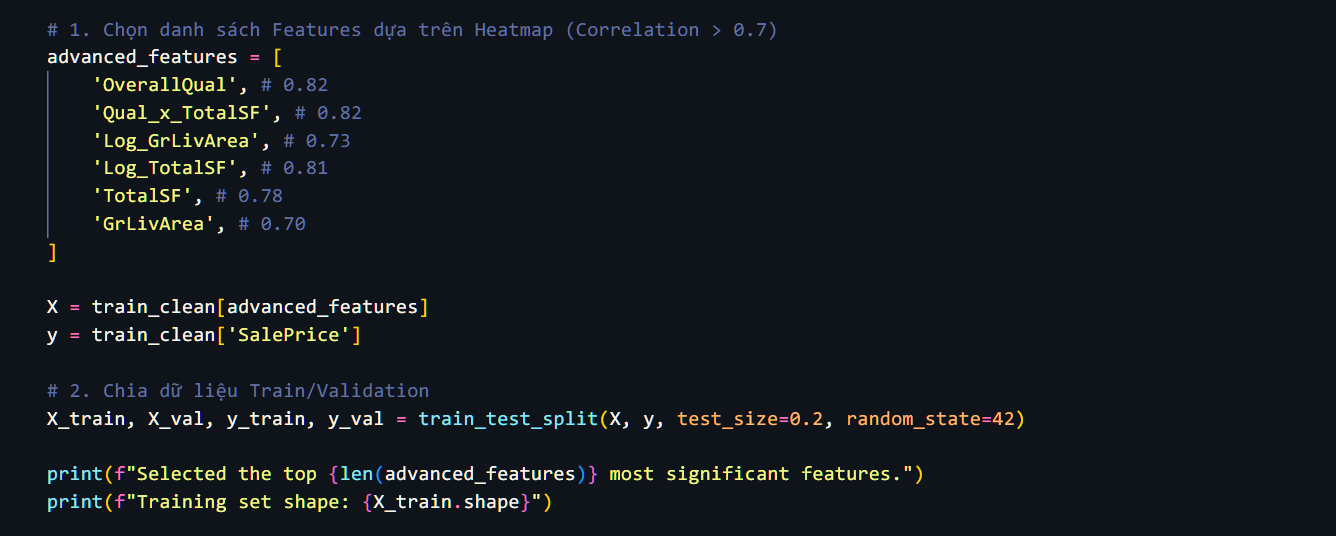
\includegraphics[width=1\linewidth]{images/advanced_model/SplitData.png}
    \caption{Chia dữ liệu thành training và validation set}
\end{figure}

\subsection{Kết quả đánh giá mô hình nâng cao}
